% \begin{table*}[t]
\centering
\caption{$M_{miss}$ and $M_{remain}$ for \tool with the increases of entry nodes}
\label{tab:toolReductionAndMissing}
\resizebox{\textwidth}{!}{
\begin{tabular}{crrrrrrrrr}
\hline
%rowcolor[HTML]{C0C0C0} 
\textbf{Attack}        & \multicolumn{1}{c}{\textbf{1-$M_{miss}$}} & \multicolumn{1}{c}{\textbf{1-$M_{remain}$}} & \multicolumn{1}{c}{\textbf{1-$\# Edge$}} & \multicolumn{1}{c}{\textbf{2-$M_{miss}$}} & \multicolumn{1}{c}{\textbf{2-$M_{remain}$}} & \multicolumn{1}{c}{\textbf{2-$\# Edge$}} & \multicolumn{1}{c}{\textbf{3-$M_{miss}$}} & \multicolumn{1}{c}{\textbf{3-$M_{remain}$}} & \multicolumn{1}{c}{\textbf{3-$\# Edge$}} \\ \hline
Wget Executable      & 0.00                                                                      & 0.0413                                                                    & 15.00                                                                     & 0.00                                                                         & 0.1350                                                                   & 49                                                                        & 0.00                                                                      & 0.1460                                                                      & 53.00                                                                     \\ 
%rowcolor[HTML]{C0C0C0} 
Illegal Storage      & 0.17                                                                      & 0.0010                                                                    & 63.00                                                                     & 0.00                                                                         & 0.0011                                                                   & 67                                                                        & 0.00                                                                      & 0.0012                                                                      & 77.00                                                                     \\ 
Illegal Storage 2    & 0.00                                                                      & 0.0016                                                                    & 604.00                                                                    & 0.00                                                                         & 0.0016                                                                   & 607                                                                       & 0.00                                                                      & 0.0017                                                                      & 628.00                                                                    \\ 
%rowcolor[HTML]{C0C0C0} 
Hide File            & 0.08                                                                      & 0.0002                                                                    & 800.00                                                                    & 0.00                                                                         & 0.0002                                                                   & 805                                                                       & 0.00                                                                      & 0.0002                                                                      & 809.00                                                                    \\ 
Steal Information    & 0.00                                                                      & 0.0002                                                                    & 821.00                                                                    & 0.00                                                                         & 0.0003                                                                   & 854                                                                       & 0.00                                                                      & 0.0003                                                                      & 858.00                                                                    \\ 
%rowcolor[HTML]{C0C0C0} 
Backdoor Download    & 0.00                                                                      & 0.0009                                                                    & 55.00                                                                     & 0.00                                                                         & 0.0010                                                                   & 59                                                                        & 0.00                                                                      & 0.0021                                                                      & 129.00                                                                    \\ 
Annoying Server User & 0.00                                                                      & 0.0409                                                                    & 13.00                                                                     & 0.00                                                                         & 0.0660                                                                   & 21                                                                        & 0.00                                                                      & 0.0755                                                                      & 24.00                                                                     \\ 
%rowcolor[HTML]{C0C0C0} 
Shellshock           & 0.00                                                                      & 0.0719                                                                    & 33.00                                                                     & 0.00                                                                         & 0.1068                                                                   & 49                                                                        & 0.00                                                                      & 0.1089                                                                      & 50.00                                                                     \\ 
Dataleak             & 0.00                                                                      & 0.0742                                                                    & 17.00                                                                     & 0.00                                                                         & 0.1048                                                                   & 24                                                                        & 0.00                                                                      & 0.1135                                                                      & 26.00                                                                     \\ 
%rowcolor[HTML]{C0C0C0} 
VPN Filter            & 0.00                                                                      & 0.0287                                                                    & 19.00                                                                     & 0.00                                                                         & 0.0378                                                                   & 25                                                                        & 0.00                                                                      & 0.0408                                                                      & 27.00                                                                     \\ 
\textbf{AVG}         & 0.02                                                                      & 0.0261                                                                    & 244.00                                                                    & 0.00                                                                         & 0.0455                                                                   & 256                                                                       & 0.00                                                                      & 0.0490                                                                      & 268.10                                                                    \\ \hline
\end{tabular}
}
\end{table*}
% \input{tables/s&p/rq2random.tex}

\begin{figure}[t]
    \centering
    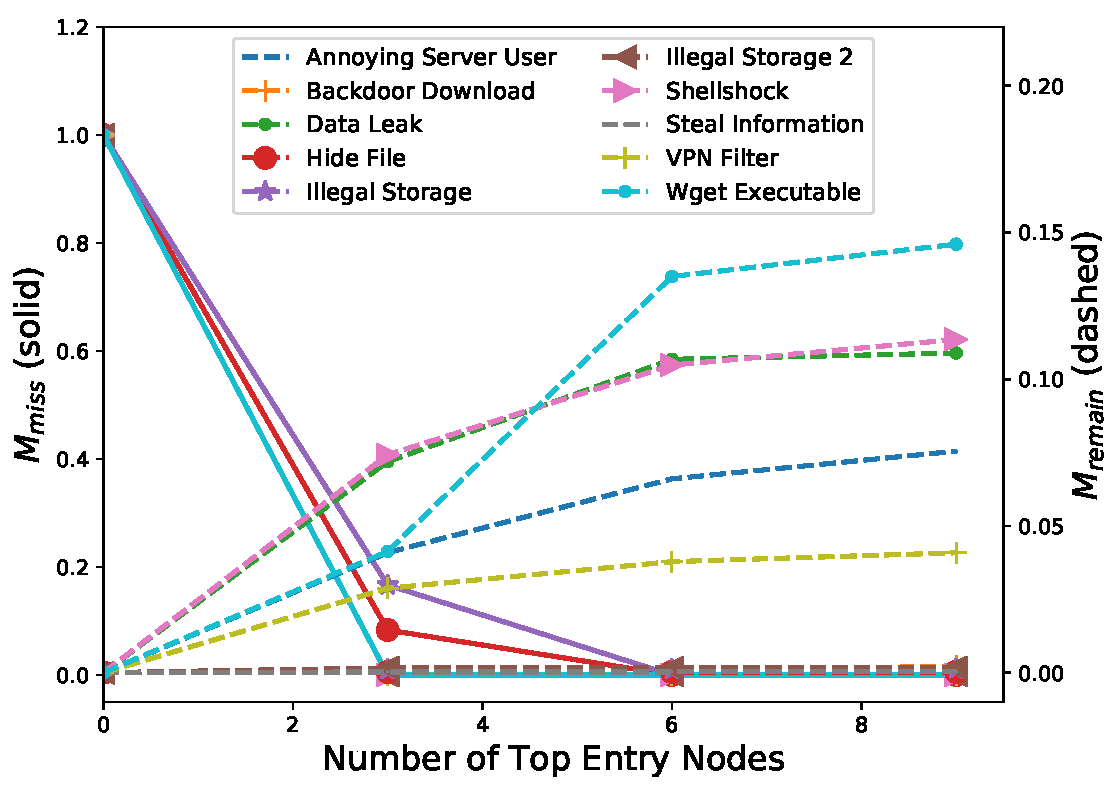
\includegraphics[width=0.47\textwidth]{figs/s&p/rq2-crop.pdf}
    \caption{$M_{miss}$ and $M_{remain}$ using top-ranked entry nodes by considering 3 types of system entities (3, 6, 9 nodes)}
    \label{fig:rq2batch}
\end{figure}
\begin{figure}[t]
    \centering
    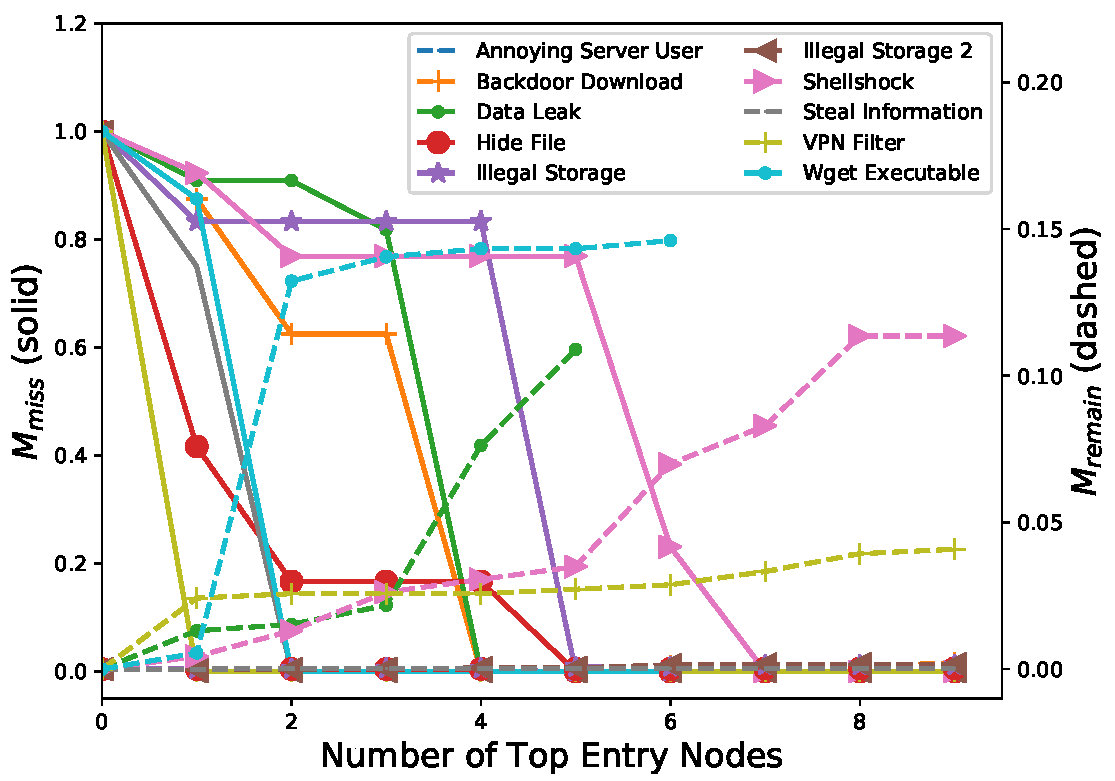
\includegraphics[width=0.47\textwidth]{figs/s&p/rq2m-crop.pdf}
    \caption{$M_{miss}$ and $M_{remain}$ using top-ranked entry nodes without considering the types of system entities (1-9 nodes)}
    \label{fig:rq2single}
\end{figure}

\subsection{RQ2: Impacts of Top-Ranked Entry Nodes}
\label{subsec:rq2}
% Given a dependency graph from a POI event, \tool chooses a number of top-ranked nodes to perform forward causality analysis, and remove the edges that cannot be found via the forward causality analysis.
Intuitively, the more entry nodes \tool uses to perform forward causality analysis, the less likely \tool will incorrectly filter out critical edges.
However, more entry nodes will also cause more non-critical edges to be preserved in the final output graph.
%(\ie overlap of the forward dependency graph and the original backward dependency graph). 
To demonstrate the effectiveness of selecting the top-ranked entry nodes in revealing attack sequences, we show how the increase of the selected top-ranked entry nodes impact the effectiveness of \tool in preserving critical edges and filtering out non-critical edges.
As attack entries may be from different types of system entities, we also compare the effectiveness of two mechanisms in selecting top-ranked entry nodes: one considers the types of system entities and the other does not.

% we first compare \tool with a random approach that randomly selects entry nodes to perform forward causality analysis for filtering. 
% For \tool, we choose top 1, top 2, and top 3 entry nodes from the 3 types of system entities to perform the graph reduction. 
% For the random approach, we choose the 3, 6, and 9 entry nodes for fair comparison.


\myparatight{Evaluation Metrics}
To measure the missing of critical edges, we compute the \emph{missing rate} $M_{miss} = N_{miss} / N_{critical}$, where $N_{miss}$ represents the number of missing critical edges and $N_{critical}$ represents the total number of critical edges (Column ``Critical Edge'' in \cref{tab:stasticalSummary}).
%
To measure the effectiveness of graph reduction, we compute the \emph{remaining rate} $M_{remain} = N_{remain} / N_{total}$, where $N_{remain}$ represents the number of edges in the output graph 
%generated by \tool 
and $N_{total}$ represents the number of edges in the dependency graph after the edge merge (Column ``Edge Mer. \# E'' in \cref{tab:stasticalSummary}).


\eat{
\myparatight{Comparison to Random Approach}
\cref{tab:toolReductionAndMissing} and \cref{tab:rq2random} show the comparison results.
Columns ``1-$M_{miss}$'', ``1-$M_{remain}$'', and ``1-$\# Edge$'' show the average value of $M_{miss}$, the average value of $M_{remain}$, and the average number of edges in the final graph for \tool and the random approach by using the top 1 entry nodes of the 3 types of system entities.
Columns ``2-$M_{miss}$'', ``2-$M_{remain}$'', ``2-$\# Edge$'', ``3-$M_{miss}$'', ``3-$M_{remain}$'', and ``3-$\# Edge$'' show the same metrics for the top 2 and the top 3 entry nodes, respectively. 

As we can see, when the number of entry nodes increases, $M_{miss}$ decreases from $0.02$ to $0.00$ for \tool, but $M_{miss}$ fluctuates for the random approach. 
Another important fact is that when using more entry nodes, the average number of edges remained in the final graph increases from $244.00$ to $268.10$ for \tool, 
while the average number of edges increases from $31,092.21$ to $654,683.47$ for the random approach, which is significantly larger. 
% After the reduction, \tool has about hundreds of edges, but the graph processed by the random approach still has more than 30,000 edges on average. 
Compared with the random approach, \tool can further reduce the edges produced by the random approach by $99.21\%$, $99.96\%$ and $99.95\%$ using the top 1, top 2, and top 3 entry nodes, respectively.
Note that this improvement is not at the cost of losing critical edges for attacks. 
If \tool uses 6 entry nodes (\ie top 2 entry nodes from the 3 system entities), $M_{miss}$ drops to $0.0$.
These results indicates that using irrelevant entry nodes found by the random approach to perform forward causality analysis for filtering is ineffective and may cause the loss of critical edges,
while the top-ranked entry nodes found by \tool contain attack entries so that \tool is effective in revealing attack sequences. 
}

% At the same time, the total number of the edge in the critical component is $268.10$ on average, when \tool uses all the top-three entry nodes. 
% For the random approach, this number is $654,683.47$. 

\myparatight{Impacts on $M_{miss}$ and $M_{remain}$}
As there are 3 types of system entities (\ie processes, files, and network connections), \tool uses the top-ranked entry nodes in different system entity categories
%from all the system entity types 
to perform forward causality analysis (\ie special treatment in \cref{subsubsec:entry-ranking}). 
\cref{fig:rq2batch} shows the values of $M_{miss}$ and $M_{remain}$ with the increases of the used entry nodes.
As expected, when more entry nodes are used, $M_{miss}$ decreases while $M_{remain}$ increases.
This is because performing the forward causality analysis from more entry nodes will make the final graph overlap larger, which is likely to include more critical edges and more non-critical edges. 
We can clearly see that when 6 entry nodes are used (2 nodes from each of the 3 system entity categories), $M_{miss}$ becomes $0.0$.
We further confirm that these 6 entry nodes cover all the attack entries, and more entry nodes merely contribute to the increase of $M_{remain}$.
Another finding is that the dependency impact of the node ranked at the third is about $70\%$ of the top 1 node's dependency impact.
Thus, alternatively, we can use $70\%$ of the top 1 node's dependency impact as the threshold to choose the top-ranked entry nodes for filtering.


\myparatight{Comparison of Two Selection Mechanisms for Top-Ranked Entry Nodes}
We compare \tool's entry node selection mechanism with another mechanism that does not consider system entity categories (\ie selecting top-ranked entry nodes based on their dependency impacts directly).
\cref{fig:rq2single} shows the values of $M_{miss}$ and $M_{remain}$ for this mechanism.
As we can see, for some attacks (\eg the ``VPNFilter'' and ``Wget Executable'' attacks), $M_{miss}$ becomes $0.0$ when the top 1 and the top 2 entry nodes are used,
but some attacks (\eg the ``Shellshock'' attack) requires 7 entry nodes for $M_{miss}$ to become $0.0$.
On the contrary, for all the attacks, the selection mechanism that considers system types can ensure zero-loss of critical edges when 6 entry nodes are used.

\myparatight{Summary}
These results indicate that (1) the top-ranked nodes provided by \tool are effective in preserving critical edges and reducing non-critical edges when the top 2 entry nodes from the 3 types of system entities are used;
(2) the mechanism that considers the types of system entities when choosing the top nodes achieves more stable results for different type of attacks than the one without considering the types of system entities.







\eat{
Considering the complexity of the potential cyberattack, if users want to include more entry points for forward reduction, the change rate of relevance score can be a useful
threshold that may help users select entry node candidates. 
According to our current results, the suggested threshold value for relevance score change is $28\%$. 
That means users can select entry nodes, whose relevance score is bigger than $72\%$ of the highest relevance score in the corresponding category, to do the forward analysis.
}



\eat{

These results demonstrate the superiority of \tool over the random approach,
which is mainly due to the better selection of the entry nodes.
For \tool, the selection of entry nodes is based on the relevance score ranking. 
For the random approach, this selection is a random decision. 
Based on this finding, we can conclude the effectiveness of the graph reduction highly depends on the selection of entry nodes. 


$M_{size}$ is used to measure the graph reduction rate, which is defined as:
\begin{equation}
    M_{size} = \frac{N_{critical}}{N_{merge}}
\end{equation}
$N_{critical}$ is the number of edges in the critical component generated by \tool. $N_{merge}$ is the number of edges after the edge merges. 
A good reduction method should have a small $M_{size}$. If we don't do any graph reduction, $M_{size}$ will be $1.0$.

$M_{miss}$ is used to measure the information loss during the graph reduction. 
Because the corresponding information is represented as edges in dependency graph, we use the critical-edge missing rate to measure the attack information loss. 
$M_{miss}$ is defined as:
\begin{equation}
    M_{miss} = \frac{N_{missing}}{N_{total}}
\end{equation}
$N_{missing}$ is the number of missing critical edges in the critical component generated by \tool. Since we have control over the test environment of these attack cases, we are able to figure out the ground truth of the attack sequences. 
We have the total number of critical edges that should be contained by the critical component, which is represented by $N_{total}$.
Without any filtering, the dependency graph constructed via performing a backward causality analysis from a POI has the $M_{miss}$ being $0.0$.



\tool chooses the top-ranked entry nodes to perform forward causality analysis, and filter the edges that do not appear in the forward causality analysis. 
For this evaluation, we choose the top 3 entry nodes of each category as candidates, and thus we have 9 nodes as candidates in general. 
Given these candidate nodes, we assume that users may pick any of these 9 nodes to perform forward causality analysis for reduction. 
In this evaluation, we use a straightforward way to add entry nodes for forward reduction. 
We add a batch of entry nodes including all 3 kinds of system entities (\ie file, process and IP), the order is according to the rank of relevance score.
Thus, we compute the $M_{size}$ by allowing users to select all top1, top2, or top3 nodes among these candidates, respectively, and then compute $M_{miss}$.


To demonstrate the effectiveness of \tool's graph reduction, we compare \tool with the random  approach. 
For the random approach, all the entry nodes are candidates and the entry nodes used to do the graph reduction are randomly selected. 
We run the random approach for 20 times and compute the average result for these metrics.
For fairness, we will compare the results of \tool and the random approach with the same number of selected nodes, respectively.
}

% We evaluate the graph reduction and critical-edge missing rate, when the attack investigation uses different number of candidates to do the forward reduction. 
% For the dependency graph reduction, if we just simply remove 99.99\% edges of dependency graph, we may have a small graph can be easily analyzed, but it is very possible that we lose all the information about attack. 
% If we only pursue to keep all the attack information, the safest reduction way is just keep all the edges. 
% However, this graph is still too large to be analyzed. 
% The ideal method is try to keep all the critical edges, at the same time remove as much irrelevant edges to POI event as possible.